\documentclass[a4paper, 12pt]{article}
\usepackage[utf8]{inputenc}
\usepackage{graphicx}
\usepackage[norsk]{babel}
\usepackage{subfigure}

\begin{document}

\title{Prosjektkravspesifikasjon for Genyx}
\author{Marius Geitle}
\date{\today}

\maketitle
\tableofcontents
\listoffigures

\section{Introduksjon}
\subsection{Formål}
Formålet med dette dokumentet er å gi en detaljert beskrivelse av kravene til
"Genyx". Det vil illustrere formålet av systemet, og illustrere begrensningene,
grensesnittene og interaksjon med ekstern programvare. Dette dokumentet er ment for å
bli presentert for Lars Emil Knudsen for godkjenning og som referanse for utvikling
av første versjon.


\subsection{Omfang}
Genyx er en notat applikasjon som gjør det mulig å benytte en android enhet til å
skrive notater under møter eller andre steder og effektivt kunne finne igjen gamle
notater ved å bruke enten geografisk posisjon, tidsrom, fri-tekst søk, og/eller
kategorisering.

Under notering vil brukeren kunne opprette et notat som består av flere sider, og sidene kan inneholde enten bilder som kan bli ikke-destruktivt annotert, tekst, eller håndtegnet grafikk slik som håndskrift eller tegninger.

Applikasjonen trenger tilgang til CalendarProvider for å kunne knytte opp notater mot kalenderhendelser. Den trenger også tilgang til internett og både fin og grov posisjon for geografisk markering av notater. Det vil også bli utredet om det er hensiktsmessig å integrere med facebook for å kunne tagge notater med venner fra facebook.

\section{Overordnet beskrivelse}
\subsection{Produktperspektiv}
Applikasjonen vil være en mobil applikasjon for Android enheter. Mobilapplikasjonen blir brukt til å behandle, se, og redigere notater og behandle kategorilister.

Applikasjonen vil benytte en lokal SQLite database for lagring av notater, kategorilister ol.

For å tagging av notater med informasjon om hvilen kalenderhendelse dette notatet gjelder så vil applikasjonen benytte android API for tilgang til den innebygde kalenderdatabasen.

For visning av kart og geografisk tagging av notater vil en geografisk posisjonering  bli utført både ved hjelp av det mobile nettverket og GPS.

Kamera vil bli benyttet for import av bilder til notater.

\subsection{produktfunksjoner}
Applikasjonen vil gjøre det mulig å opprette og redigere eksisterende notater som blir lagret i en lokal database på den mobile enheten. Notatet vil kunne bestå av flere sider som igjen er splittet opp i lag. Et lag kan bestå av bilde, kart, tekst, eller hånd-tegnet grafikk. Notater kan også inneholde bilder og andre filer som vedlegg, ved åpning av vedlegg vil den applikasjonen på enheten som er registrert for den aktuelle filtypen bli benyttet. Notatet kan bli merket med en eller flere kategorier, og med geografisk posisjon. Posisjonen vil kunne merkes enten ved hjelp av manuell markering på kart, ved hjelp av mobilnett for å hente posisjon, eller ved å benytte GPS.

Med applikasjonen så vil brukeren kunne søke opp gamle notater ved hjelp av flere søkekriterier, deriblant avstand fra et punkt på et kart, fri-tekst, og kategori. Resultatene vil kunne bli vist enten på kart, eller i listeform.

Listen med kategorier som brukeren kan markere notater med vil kunne bli behandlet og det vil være mulig å slette, redigere og opprette nye kategorier.

\subsection{Brukertyper}
Denne applikasjonen vil være ment for brukere som trenger å kunne lage større notater og kunne kategorisere notatene og markere kategoriene med geografisk informasjon uten å måtte gjøre en ekstrajobb med å sette opp en ryddig struktur. Dette kan inneholde konsulenter som ofte drar på møter, landskapsfotografer som ønsker når de er ute på leting etter fotosteder kan ta referansebilder og notere ned informasjon som lyssetting osv.

En annen brukergruppe er studenter som ønsker en enkel mobilapplikasjon som kan bli brukt under forelesninger for å enkelt kunne notere ned informasjon og kunne tegne av tegninger på White Board / tavle, men ikke ønsker å bruke tid på å sette opp mappestrukturer ol.

\subsection{Begrensninger}
Denne applikasjonen vil benytte både GPS og mobilt nett for å hente ned posisjonen til brukeren, og det kan være variasjoner i hvilke posisjoneringstjenester de forskjellige mobile enhetene tilbyr, og enkelte posisjonstjenester kan være utilgjengelig enkelte steder slik som GPS er inne i bygninger.

Brukeropplevelsen av applikasjonen kan forringes ved å benytte applikasjonen på en enhet med liten skjerm, eller dårlig oppløsning da notater kan trenge å vise mye informasjon på en skjerm om gangen.

Fordi alle data blir lagret lokalt på enheten vil antall notater som kan lagres på enheten være begrenset av tilgjengelig diskplass.

\subsection{Antagelser og avhengigheter}
En antagelse som blir tatt er at de mobile enhetene er kraftige nok, og har nok tilgjengelig ytelse til å kjøre applikasjonen. Hvis enheten ikke er kraftig nok til å kjøre applikasjonen så kan applikasjonen ikke fungere som ment, eller ikke i det hele tatt.

For at applikasjonen skal kunne tilby geo-lokasjonstjenester via GPS er det nødvendig at GPS er tilgjengelig på enheten. Hvis GPS ikke er tilgjengelig vil ikke denne opsjonen være tilgjengelig.

\subsection{Utelating av funksjonalitet}
For å hindre at prosjektet ikke blir ferdig er det enkelt funksjonalitet som kan bli utelatt fra prosjektet. Funksjoner som kan bli utelatt er facebook integrering, og at den grafiske redigeringen av notater kan bli forenklet.

\section{Spesifikke krav}
Denne seksjonen inneholder funksjonelle krav, og en detaljert beskrivelse av systemet.

\subsection{Krav til eksterne grensesnitt}
Denne seksjonen beskriver krav til all input og output fra applikasjonen.

\subsubsection{Brukergrensesnitt}

\begin{figure}[hb]
	\centering
	\subfigure[Hjem skjerm]{%
		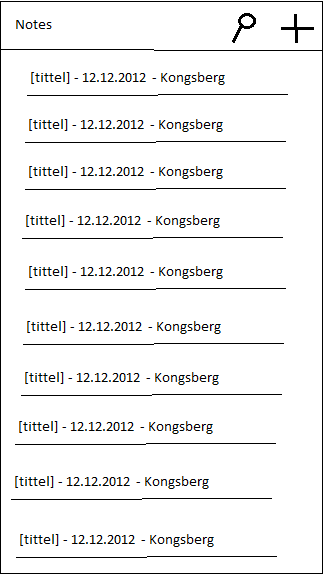
\includegraphics[width=150pt]{HomeScreen.png}
		\label{fig:homescreenfigure}}
	\quad
	\subfigure[Notatfilter skjerm]{%
		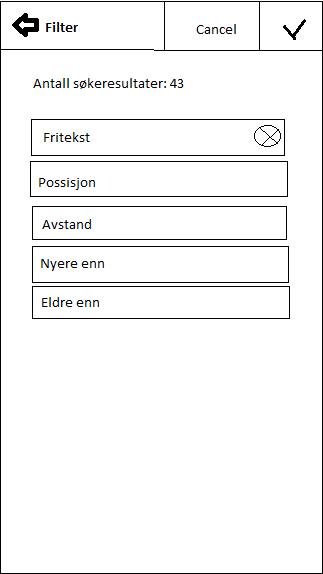
\includegraphics[width=150pt]{NoteListFilterScreen.png}
		\label{fig:NoteListFilterScreen}}
	\quad
	\subfigure[Behandle kategorier]{%
		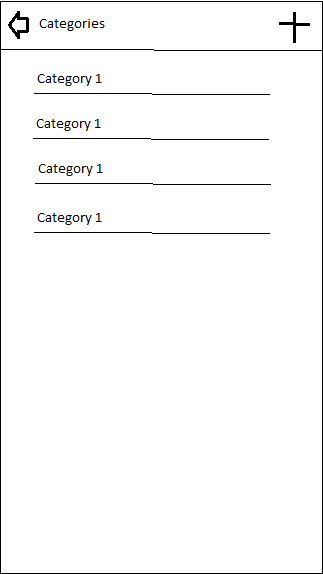
\includegraphics[width=150pt]{CategoriesScreen.png}
		\label{fig:categoriesScreen}}
	\quad
	\subfigure[Notat vedleggliste]{%
		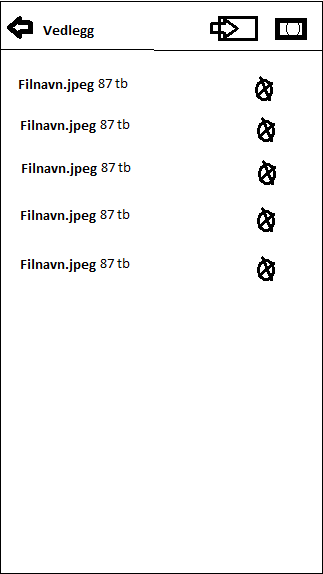
\includegraphics[width=150pt]{NoteAttachmentsScreen.png}
		\label{fig:NoteAttachmentsScreen}}
	%
	\caption{Skjermer}
\label{fig:screens}
\end{figure}

\begin{figure}[hb]
	\centering
	\subfigure[Vis notat]{%
		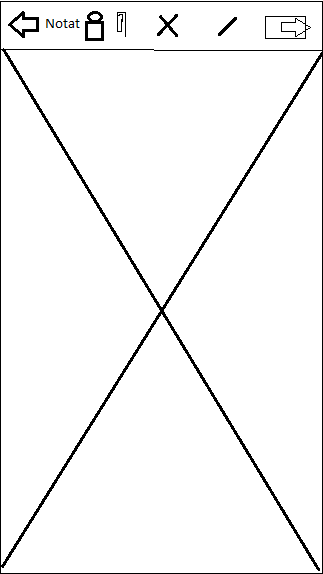
\includegraphics[width=150pt]{NoteViewScreen.png}
		\label{fig:NoteViewScreen}}
	\quad
	\subfigure[Rediger notat]{%
		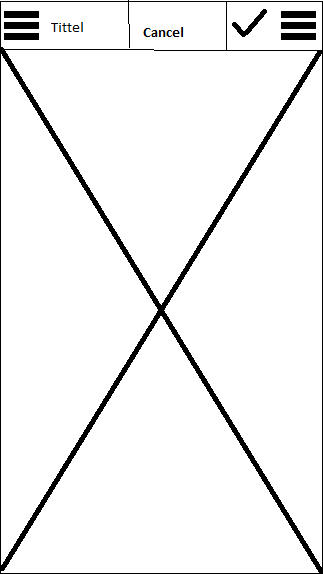
\includegraphics[width=150pt]{NoteEditScreen.png}
		\label{fig:NoteEditScreen}}
	\quad
	\subfigure[Rediger notatside skjerm]{%
		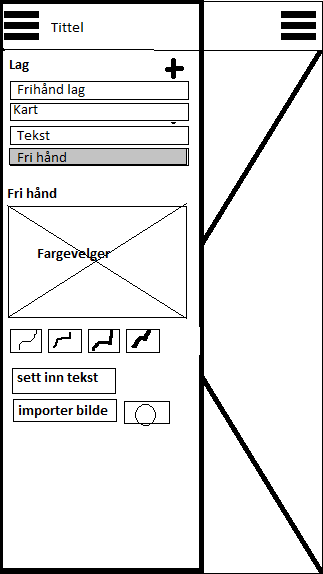
\includegraphics[width=150pt]{NoteEditPageScreen.png}
		\label{fig:NoteEditPageScreen}}
		\quad
	\subfigure[Rediger notatmeta skjerm]{%
		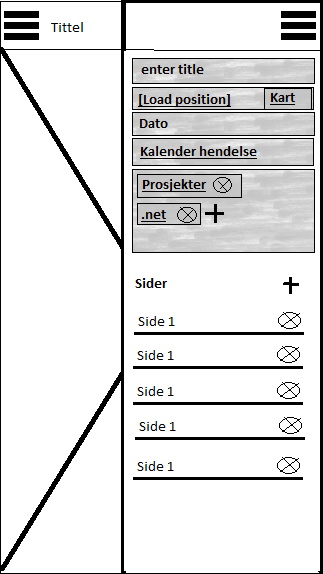
\includegraphics[width=150pt]{NoteEditNoteScreen.png}
		\label{fig:NoteEditNoteScreen}}
	%
	\caption{Notatskjermer}
\label{fig:notescreens}
\end{figure}


\paragraph{Hjemskjermen} (Se Figur \ref{fig:homescreenfigure} på side~\pageref{fig:homescreenfigure}) vil inneholde en liste over alle notatene, sortert med de nyeste først. Den vil implementere lazy loading av elementer slik at ikke alle elementer lastes samtidig. Hvert listeelement inneholder tittelen på notatet, og stedet den ble registrert (hvis tilgjengelig). Og datoen den sist ble modifisert. Når brukeren holder fingeren på notatet i en lengre periode så blir brukeren spurt om å slette notatet. Ved å trykke på kontekst meny knappen på telefonen vil brukeren få opp en meny med mulighet til å gå til en "About"~skjerm, og mulighet for å behandle kategorilisten. Listen med notater kan filtreres ved å trykke på filtreringsknappen som navigerer brukeren til Filterskjermen.

\paragraph{Filterskjermen} (Se Figur \ref{fig:NoteListFilterScreen} på side~\pageref{fig:NoteListFilterScreen}) her vil brukeren kunne legge inn filter på fritekst, avstand fra et geografisk punkt, og dato. En teller over antall søkeresultater oppdateres ved endring av filterkriteria.

\paragraph{Behandle~kategorier~skjermen}(Se Figur \ref{fig:categoriesScreen} på side~\pageref{fig:categoriesScreen}) vil inneholde en liste over alle kategoriene. For å opprette en ny kategori benyttes + knappen. For å slette en kategori så blir brukeren presentert med et spørsmål om å slette kategorien hvis brukeren peker på kategorien i en lengre periode.

\paragraph{Notatskjermen} Når brukeren går inn på et eksisterende notat så blir brukeren presentert med en kun-lese visning av notatet. Der er det mulighet for å sende til andre enheter ved å trykke på sendeikonet, brukeren må da velge hvilken måte notatet skal sendes på. Alternativer vil da være PDF over epost, og andre som vil bli vurdert på et senere tidspunkt, og ved å trykke på sletteknappen kan brukeren slette notatet. Brukeren kan også se og redigere listen over vedlegg fra vedlegg knappen (binders) som fører til at brukeren blir navigert til vedlegglisten. Brukeren kan også ved å trykke på silhuetten av en person tagge personer som har tilknytning til notatet. ved å trykke på pennikonet så ender brukeren opp i redigeringsmodus (Se Figur \ref{fig:NoteEditScreen} på side~\pageref{fig:NoteEditScreen}). som vil vise alle lagene i det viste notatet uten noen synlige menyer, hvis det er et nytt nytt notat vil notatet inneholde et tomt fri-hånd lag. Alternativ menyen vil inneholde knapp for sletting av notatet. Ved trykking på den venstre menyknappen vil brukeren få opp meny en meny for redigering av den aktive siden i notatet (se Figur \ref{fig:NoteEditPageScreen} på side~\pageref{fig:NoteEditPageScreen}). I denne pop-out menyen så vil det på toppen være en liste over alle lagene i den aktuelle siden. Ved å trykke på laget blir laget valgt, og kan redigeres. Opprettelse av nytt lag blir gjort ved å trykke på + til høyre for overskriften til regionen. Brukeren må da velge i en dialog hvilken type lag som skal legges til. Når et fri-hånd-lag er valgt så kan brukeren også velge farge på penn, og tykkelse på linjene. Brukeren kan også velge å sette inn tekst i tegningen, importere et bilde fra galleri, eller benytte kamera for å knipse et bilde. Android FaceDetection API vil bli kjørt på det importerte bilde, og hvis fjes blir oppdaget blir brukeren spurt om å tagge personer i notatet. For å redigere data felles for hele notatet så trykker brukeren på den høyre menyknappen i topplinjen. Brukeren vil da bli vist en popout meny (Se Figur \ref{fig:NoteEditNoteScreen} på side~\pageref{fig:NoteEditNoteScreen}) her vil brukeren kunne legge inn tittel, dato, geografisk lokasjon, koble til kalenderhendelse, og spesifisere kategorier, og legge til og fjerne notatsider. Redigering av tittel er et normalt textView. For å redigere den geografiske posisjonen så vil man når man trykker på feltet kunne velge om posisjon skal lastes fra GPS eller basert på mobilnett. Det er også mulig å velge finne posisjonen påved hjelp av et kart ved å trykke på "kart" knappen. Når man skal redigere dato blir brukeren vist en android DatePicker for å velge dato. For å velge kalenderhendelse så blir brukeren vist en liste over hendelser fra alle kalendere som er tilgjengelige via Calendar Provider. Hvis kalenderhendelen er knyttet til flere personer blir brukeren spurt om de personene skal tagges i notatet. For å legge til en ny kategori så blir brukeren vist en dialog for å velge kategori eller opprette nye kategorier ved å trykke på + knappen som er plassert etter den siste kategorien. For å velge aktiv side så kan brukeren velge siden i listen. Det vil også være mulig å slette sider ved å trykke på sletteknappen og opprette nye sider ved å trykke på +. Ved opprettelse av ny side blir brukeren spurt om sidetype med standard valgt fri-hånd.

\paragraph{Notatvedleggskjerm} (Se Figur \ref{fig:NoteAttachmentsScreen} på side~\pageref{fig:NoteAttachmentsScreen}) vil brukeren kunne redigere hvilke vedlegg som ligger ved på notatet. Ved å trykke på kamera-ikonet vil kamera starte, og bilde vil etterpå bli importert inn i notatet. Ved å trykke på import knappen vil brukeren kunne velge en fil fra filsystemet for import inn i notatet. Når et vedlegg blir trykt på blir det åpnet i det programmet som er registrert av android for å kunne åpne den filtypen, unntaket fra dette er bildefiler som blir vist inne i applikasjonen. Vedlegget kan slettes ved å trykke på krysset i listen.

\paragraph{Widget} vil vise de siste notatene med lazyloading for å kunne scrolle igjennom alle. Listen vil vise de siste notatene i nærheten av nåværende plassering, og vil inneholde en snarvei for opprettelse av nye notater. Visningen er kan bli konfigurert for hvor ofte listen skal oppdateres og om den skal aktivt hente geografisk posisjon med standard at den skal hente posisjon passivt. Dvs. når andre programmer henter inn posisjonen.

\subsubsection{Maskinvaregrensesnitt}
Applikasjonen vil være avhengig av GPS, og vil benytte android GPS subsystem for kommunikasjon med GPS enheter, og kamera API for integrasjon med kommunikasjon med kamera.

\subsubsection{Programmvaregrensesnitt}
For å hente inn den geografiske posisjonen til brukeren vil applikasjonen benytte mobilt nettverk, GPS, and evt. andre metoder for å hente den aktuelle posisjonen til brukeren. For å gjøre dette vil android geo navigasjon subsystemet bli benyttet. Kamera blir benyttet for å kunne knytte et bilde til et notat som blir importert enten som et vedlegg til notatet, eller som en tegning i et fri-hånd lag.

\subsubsection{Kommunikasjonsgrensesnitt}
Applikasjonen vil måtte kommunisere for å sende notater til andre enheter. For å sende notat til andre enheter er via epost en opsjon. For kommunikasjon via epost vil standard epostklient bli benyttet. Det vil også på et senere tidspunkt bli utredet for muligheter til å benytte Bluetooth(tm) og NFC.

\end{document}